\chapter{软件设计与分析}

\section{软件架构设计}\label{sec:architecture}

农业果实称重云端软件的整体架构采用边端+远端协同的模式进行设计,将靠近农场端的服务称为边端服务,远离农场端的服务称为远端服务,其中边端服务一般部署在农场局域网内,在网络受限的情况下,确保称重流程的正常进行。整体软件部署架构图如图\ref{fig:软件部署架构图}所示。

\begin{figure}[H]
    \centering
    \includegraphics[width=0.8\linewidth]{../design/out/软件部署架构图.png}
    \caption{软件部署架构图}
    \label{fig:软件部署架构图}
\end{figure}

如图\ref{fig:软件部署架构图}所示,存在三个端,分别是边端、远端以及前台网页端,它们分别部署在三台不同服务器上。电子秤提交称重数据的通信流程如下:

1、不同类型的电子秤通过不同协议向网关提交称重数据;

2、网关处理电子秤的发出的请求,通过 EMQX 协议转换技术完成协议转换,通过读取 MySQL 从库数据完成电子秤信息认证和授权,最后将数据以 MQTT 协议的格式发送至 MQTT Broker 集群;

3、MQTT Broker 接收到 MQTT 消息后,该集群内任一节点都可以处理请求并将消息持久化;

4、远端服务订阅 MQTT Broker 集群中所有节点的消息,收到消息后进行消息解析,通过果实识别服务识别出果实种类,然后将称重结果写入 MySQL 主库;

5、至此已经完成称重数据的处理。此外,在前台网页端,员工可以查看历史称重记录,管理员可以在待办界面处理待办,手动填写并提交处理失败的称重数据。

进一步分析软件架构的特点,可以得到软件的分层架构图,如图\ref{fig:软件分层架构图}所示。

\begin{figure}[H]
    \centering
    \includegraphics[width=0.8\linewidth]{../design/out/软件分层架构图.png}
    \caption{软件分层架构图}
    \label{fig:软件分层架构图}
\end{figure}

软件可以抽象出五个层级,分别是表现层、通信层、网关层、服务层、数据层。各层作用如下:

1、表现层:该层可以理解为接口调用者,包含前台网页端和电子秤,两者都通过调用后台提供的接口来完成数据的处理或展示;

2、通信层:该层服务于表现层和网关层之间的通信。软件所支持的通信协议有四种,分别是 HTTP/HTTPS、MQTT、CoAP 和 STOMP。其中前台网页端可以通过 HTTP/HTTPS 调用后台接口,而电子秤可以通过四种协议中任一一种来提交称重数据;

3、网关层:该层提供了接口路由和协议转换功能。表现层发来的请求根据接口路由导向服务层中对应的服务,协议转换功能则服务于电子秤,将不同协议统一转为 MQTT 协议,以 MQTT 协议继续进行后续通信;

4、服务层:该层完成具体的数据服务逻辑。包含四大模块,用户模块、果实模块、作业模块以及称重模块,各个模块相互依赖,共同协作,完成数据的查询和处理;

5、数据层:该层完成数据的持久化和缓存操作。MySQL 数据库用于持久化数据,Redis 数据库用于实现数据缓存功能,而 MQTT Broker 类似于消息队列,用于临时存储 MQTT 消息。

综上所述,根据软件部署架构图\ref{fig:软件部署架构图}可以得到软件整体的通信流程和部署思路,根据软件分层架构图\ref{fig:软件分层架构图}可以清晰地划分出功能模块,更高效地进行后续软件的开发。

\section{数据库设计}\label{sec:database}

本软件数据库设计分为三个阶段:概念模型设计、逻辑模型设计和物理模型设计,下面进行具体阐述。

\subsection{概念模型设计}

农业果实称重云端软件中,可以抽象出果实、称重记录、电子秤、采摘作业、用户、待办记录这六个实体对象,结合实际的业务场景,可以得到实体关系如表\ref{tab:ertab}所示。

\begin{table}[H]
\centering
\caption{实体关系表}
\label{tab:ertab}
\begin{tabular}{|c|c|c|}
\hline
关系名称 & 关系类型 & 描述 \\ \hline

采摘目标 & 1:N & 果实 1,采摘作业 N \\ \hline

称重目标 & 1:N & 果实 1,称重记录 N \\ \hline

称重人员 & 1:N & 员工 1,称重记录 N  \\ \hline

记录来源 & 1:N & 电子秤 1,称重记录 N \\ \hline

待办人员 & 1:N & 员工 1,待办记录 N \\ \hline

待办来源 & 1:N & 电子秤 1,待办记录 N \\ \hline

\end{tabular}%
\end{table}

将上述分析进行归纳,得到 ERD(Entity-Relationship Diagram, 即实体关系图)如图\ref{fig:ERD}所示。

\begin{figure}[H]
    \centering
    \includegraphics[width=0.8\linewidth]{../design/out/ERD.png}
    \caption{实体关系图}
    \label{fig:ERD}
\end{figure}

图\ref{fig:ERD}清晰地展示了各个实体之间的复杂关系,为后续进行数据库的逻辑模型设计奠定了基础。

\subsection{逻辑模型设计}

基于图\ref{fig:ERD}所展示的实体关系以及功能权限表\ref{tab:user_permissions}所展示的用户功能权限信息,下面阐述逻辑模型设计,描述系统各个表的结构及其字段定义,涵盖了表之间的关系、字段的数据类型及约束条件,如表\ref{tab:user},表\ref{tab:produce},表\ref{tab:work},表\ref{tab:scale},表\ref{tab:record},表\ref{tab:todo},表\ref{tab:mqttacl}所示。

% t_user
\begin{table}[H]
    \centering
    \caption{用户表 (t\_user)}
    \label{tab:user}
    \begin{tabular}{|l|l|l|l|}
    \hline
    字段 & 类型 & 约束 & 说明 \\
    \hline
    id & bigint & 主键 & 自增主键 \\
    uid & varchar(255) & 非空,唯一 & 用户认证编号 \\
    name & varchar(255) & 非空 & 用户名称 \\
    password & varchar(255) & 非空 & 密码(加密) \\
    roles & varchar(255) & - & 角色(英文逗号分隔) \\
    create\_time & bigint & 非空 & 创建时间(毫秒级时间戳) \\
    update\_time & bigint & 非空 & 更新时间(毫秒级时间戳) \\
    status & int & 非空 & 状态(0禁用/1启用/2已删除) \\
    \hline
    \end{tabular}
    \end{table}

表\ref{tab:user}中展现了软件中用户实体的具体字段设计,其中 roles 字段定义了用户角色,角色字段包含管理员(ROLE\_ADMIN)、采摘员工(ROLE\_EMPLOYEE)、电子秤(ROLE\_SCALE)以及系统用户(ROLE\_SYS),如果用户包含多个角色,则使用英文半角逗号隔开。

% t_produce
\begin{table}[H]
\centering
\caption{果实表 (t\_produce)}
\label{tab:produce}
\begin{tabular}{|l|l|l|l|}
\hline
字段 & 类型 & 约束 & 说明 \\
\hline
id & bigint & 主键 & 系统自带从0开始,用户添加从1000000开始 \\
name & varchar(255) & 非空,唯一 & 果实名称 \\
name\_en & varchar(255) & 唯一 & 果实英文名称 \\
create\_time & bigint & 非空 & 创建时间(毫秒级时间戳) \\
update\_time & bigint & 非空 & 更新时间(毫秒级时间戳) \\
status & int & 非空 & 状态(0未种植/1在种植/2已删除) \\
\hline
\end{tabular}
\end{table}

表\ref{tab:produce}中展现了软件中果实实体的具体字段设计。

% t_work
\begin{table}[H]
\centering
\caption{采摘作业表 (t\_work)}
\label{tab:work}
\begin{tabular}{|l|l|l|l|}
\hline
字段 & 类型 & 约束 & 说明 \\
\hline
id & bigint & 主键 & 自增主键 \\
produce\_id & bigint & 非空 & 果实编号 \\
start\_time & bigint & 非空 & 采摘开始时间(毫秒级时间戳) \\
end\_time & bigint & 非空 & 采摘结束时间(毫秒级时间戳) \\
data\_value & decimal(10,2) & - & 总的采摘称重结果 \\
unit & int & - & 称重单位(0mg/1g/2kg/3t/4lb/5oz/6ct) \\
create\_time & bigint & 非空 & 创建时间(毫秒级时间戳) \\
update\_time & bigint & 非空 & 更新时间(毫秒级时间戳) \\
status & int & 非空 & 状态(0未开始/1进行中/2已结束/3已取消/4已删除) \\
\hline
\end{tabular}
\end{table}

表\ref{tab:work}中展现了软件中采摘作业实体的具体字段设计。其中通过字段果实编号(produce\_id)关联了果实实体,字段对应果实表\ref{tab:produce}中的 id 字段。

% t_scale
\begin{table}[H]
\centering
\caption{电子秤表 (t\_scale)}
\label{tab:scale}
\begin{tabular}{|l|l|l|l|}
\hline
字段 & 类型 & 约束 & 说明 \\
\hline
id & bigint & 主键 & 自增主键 \\
sid & varchar(255) & 非空 & MQTT 用户认证编号 \\
model & varchar(255) & - & 型号 \\
max\_capacity & decimal(10,2) & 非空 & 最大量程 \\
min\_capacity & decimal(10,2) & 非空 & 最小量程 \\
unit & int & 非空 & 量程单位(0mg/1g/2kg/3t/4lb/5oz/6ct) \\
verification\_interval & int & - & 检定分度值 \\
display\_interval & int & - & 显示分度值 \\
unit\_dv & int & - & 分度值单位(0mg/1g/2kg/3t/4lb/5oz/6ct) \\
protocol & varchar(255) & - & 协议(小写,逗号分隔) \\
create\_time & bigint & 非空 & 创建时间(毫秒级时间戳) \\
update\_time & bigint & 非空 & 更新时间(毫秒级时间戳) \\
status & int & 非空 & 状态(0禁用/1启用/2已删除) \\
\hline
\end{tabular}
\end{table}

表\ref{tab:scale}中展现了软件中电子秤实体的具体字段设计。其中通过字段电子秤编号(sid)管理了用户实体,该字段对应于用户表\ref{tab:user}中的用户编号(uid)字段。

% t_record
\begin{table}[H]
\centering
\caption{称重记录表 (t\_record)}
\label{tab:record}
\begin{tabular}{|l|l|l|l|}
\hline
字段 & 类型 & 约束 & 说明 \\
\hline
id & bigint & 主键 & 自增主键 \\
work\_id & bigint & 非空 & 采摘作业编号 \\
produce\_id & bigint & 非空 & 果实编号 \\
image & varchar(255) & - & 果实图片地址 \\
employee\_id & bigint & 非空 & 员工编号 \\
scale\_id & bigint & 非空 & 电子秤编号 \\
data\_value & decimal(10,2) & 非空 & 称重结果 \\
data\_error\_margin & decimal(10,2) & - & 称量结果误差范围 \\
unit & int & 非空 & 称重单位(0mg/1g/2kg/3t/4lb/5oz/6ct) \\
data\_time & bigint & 非空 & 称重时间(毫秒级时间戳) \\
\hline
\end{tabular}
\end{table}

表\ref{tab:record}中展现了软件中称重记录实体的具体字段设计。通过字段果实编号(produce\_id)关联了果实实体,对应果实表\ref{tab:produce}中的 id 字段;通过字段采摘作业编号(work\_id)关联了作业实体,对应作业表\ref{tab:work}中的 id 字段;通过字段员工编号(employee\_id)关联了员工实体,对应用户表\ref{tab:user}中的 id 字段;通过字段电子秤编号(scale\_id)关联了电子秤实体,对应电子秤表\ref{tab:scale}中的 id 字段。

% t_todo
\begin{table}[H]
\centering
\caption{待处理称重记录表 (t\_todo)}
\label{tab:todo}
\begin{tabular}{|l|l|l|l|}
\hline
字段 & 类型 & 约束 & 说明 \\
\hline
id & bigint & 主键 & 自增主键 \\
produce\_id & bigint & - & 果实编号 \\
produce\_name & varchar(255) & - & 果实名称 \\
image & varchar(255) & - & 采摘作业图片地址 \\
employee\_id & bigint & 非空 & 员工编号 \\
scale\_id & bigint & 非空 & 电子秤编号 \\
data\_value & decimal(10,2) & 非空 & 称重结果 \\
data\_error\_margin & decimal(10,2) & - & 称量结果误差范围 \\
unit & int & 非空 & 称重单位(0mg/1g/2kg/3t/4lb/5oz/6ct) \\
data\_time & bigint & 非空 & 称重时间(毫秒级时间戳) \\
\hline
\end{tabular}
\end{table}

表\ref{tab:todo}中展现了软件中待办记录实体的具体字段设计。通过字段果实编号(produce\_id)关联了果实实体,对应果实表\ref{tab:produce}中的 id 字段;通过字段员工编号(employee\_id)关联了员工实体,对应用户表\ref{tab:user}中的 id 字段;通过字段电子秤编号(scale\_id)关联了电子秤实体,对应电子秤表\ref{tab:scale}中的 id 字段。

% t_mqtt_acl
\begin{table}[H]
\centering
\caption{MQTT 访问控制表 (t\_mqtt\_acl)}
\label{tab:mqttacl}
\begin{tabular}{|l|l|l|l|}
\hline
字段 & 类型 & 约束 & 说明 \\
\hline
id & int & 主键 & 自增主键 \\
username & varchar(255) & 非空 & MQTT 认证用户名 \\
permission & varchar(255) & 非空 & 操作权限(allow/deny,即允许/拒绝) \\
action & varchar(255) & 非空 & 操作类型(publish/subscribe/all,即发布/订阅/所有) \\
topic & varchar(255) & 非空 & 适用主题 \\
qos & int & - & 消息 QoS 级别(0,1,2) \\
retain & int & - & 是否支持发布保留消息(0否/1是) \\
\hline
\end{tabular}
\end{table}

表\ref{tab:mqttacl}中展现了软件中 MQTT 服务的访问控制条目的具体字段设计。通过字段 MQTT 认证用户名(username)管理了用户实体,对应用户表\ref{tab:user}中的 uid 字段。

数据库中每个表的设计都遵循规范化原则,以确保数据的一致性、完整性和高效性。字段的定义包括主键、唯一约束、非空约束等,考虑到更新数据的效率问题,取消了外键的设置,在后台服务中做相关数据更新的限制以确保数据一致性。

\subsection{物理模型设计}

软件使用 MySQL 作为数据库管理系统,采用 InnoDB 存储引擎,将事务隔离级别设置为可重复读,以确保数据的一致性和可靠性。下面从索引设计、数据存储与分布、数据访问控制和事务日志与恢复策略四个方面阐述物理模型设计。

索引设计方面:针对实际业务场景,基于逻辑模型设计中的表信息,设置了相关索引以提高查询更新效率,如表\ref{tab:index}所示。

% INDEX
\begin{table}[H]
\centering
\caption{索引设计表 (INDEX)}
\label{tab:index}
\begin{tabular}{|l|l|l|}
\hline
表 & 索引字段 & 说明 \\ \hline

t\_record & scale\_id & 高效查找电子秤历史称重记录 \\ \hline

t\_record & employee\_id & 高效查找员工历史称重记录 \\ \hline

t\_record & employee\_id, work\_id & 高效查找员工各采摘作业批次历史称重记录 \\ \hline

t\_record & work\_id & 高效查找各采摘作业批次历史称重记录 \\ \hline

t\_work & produce\_id & 高效查找果实对应的采摘作业 \\ \hline
\end{tabular}
\end{table}

数据存储与分布方面:采用主从架构,在靠近农场边端部署从库,在远端服务器部署主库,主从库采用\ref{sec:gtid}中提到的基于 GTID 的主从复制技术完成数据实时同步。

数据访问控制方面:主库允许读写,而从库只允许读,屏蔽任何用户的写操作,确保数据一致性。

事务日志与恢复策略方面:主从库均开启 BinLog(二进制日志)。在上述数据复制技术中,从库通过读取主库的二进制日志来同步数据。除此之外,在数据丢失或损坏的情况下,通过回放二进制日志来恢复丢失的数据。

\section{关键功能设计}\label{sec:keyFunction}

\subsection{称重数据处理流程设计}

称重数据处理作为软件中的核心功能,这里对其进行更为详细的设计与分析。如图\ref{fig:称重数据处理流程活动图}所示。

\begin{figure}[H]
    \centering
    \includegraphics[width=0.8\linewidth]{../design/out/称重数据处理流程活动图.png}
    \caption{称重数据处理流程活动图}
    \label{fig:称重数据处理流程活动图}
\end{figure}

市面上的电子秤支持多种通信协议。对于支持 TCP/IP 的物联网设备,可以通过 WIFI、蜂窝网络以及以太网,使用 HTTP、MQTT、CoAP、LwM2M 以及 XMPP 等应用层协议协议接入云端。

网关协议是适用于短距通信无法直接上云的协议,比如蓝牙、ZigBee、LoRa 等。此类设备需要接入网关转换之后,通过 TCP/IP 协议进行上云。

本系统不考虑网关协议,只考虑应用层协议。系统将支持不同种类的电子秤,支持包含 HTTP、MQTT、MQTT-SN、CoAP、STOMP 在内的多种物联网通信协议。

为了降低开发成本,除了 HTTP、MQTT 这两种通信协议,其它物联网协议采用网关转换的方法来提供支持,网关将对各类协议转换成 MQTT 协议与 MQTT Broker 进行通信,认证规则和消息的持久化规则遵循 MQTT 协议标准。

MQTT(Message Queuing Telemetry Transport)即消息队列遥测传输协议,是一种轻量级的发布/订阅模式的消息传输协议。在电子秤系统中,发送 MQTT 消息上传称重信息具有以下优势:

一、低带宽和低功耗:MQTT 协议非常适合在低带宽和低功耗的环境下使用。对于电子秤等物联网设备来说,通常需要在有限的网络资源和电池电量下进行数据传输。MQTT 协议通过采用轻量级的消息格式和高效的发布/订阅模式,可以大大降低网络带宽的占用和设备的功耗。例如,在一些偏远地区或者移动环境下,网络带宽可能非常有限,此时使用 MQTT 协议可以确保电子秤能够及时上传称重信息,同时不会对网络造成过大的负担\cite{Jia2015}。

二、实时性和可靠性:MQTT 协议支持 QoS(Quality of Service)级别,可以根据不同的应用需求,选择不同的消息传输质量级别。在 MQTT 协议中,QoS 有三种级别\cite{Jia2015},分别是:

1、QoS0 – “最多一次”:消息最多传送一次,不保证消息到达目标。适用于实时性要求非常高,但对消息丢失容忍的场景。

2、QoS1 – “至少一次”:保证消息至少传送一次,但可能会重复。适用于需要消息可靠到达,但不介意重复接收的情况。

3、QoS2 – “只有一次”:确保每条消息只会传送一次,且无重复。适用于对消息的唯一性和可靠性有较高要求的场景。

对于需要实时上传称重信息的场景,可以选择 QoS1 或 QoS2 级别,确保消息的可靠传输。同时,MQTT 协议的发布/订阅模式可以实现实时的数据推送,当电子秤上传称重信息后,订阅了该主题的客户端可以立即收到消息,实现实时的数据更新。

三、易于扩展和集成:MQTT 协议具有良好的扩展性和集成性。可以很容易地与其他物联网协议和技术进行集成,如 CoAP、HTTP、WebSocket 等。同时,MQTT 协议的发布/订阅模式可以支持大规模的设备连接和数据传输,适用于构建物联网应用平台。例如,在智慧农业大棚测控系统中,采用 MQTT 协议将智慧大棚测控系统和阿里云物联网平台结合在一起,通过手机 APP 或 PC 软件访问阿里云服务器数据库,实现了移动终端对农业大棚实时监测和控制\cite{Liang2020}。

\subsection{果实图像识别功能设计}

农业果实称重云端软件基于 YOLOv8 实现果实图像识别功能。

采用数据集:Kaggle Fruits-360

训练结果:

\begin{figure}[H]
    \centering
    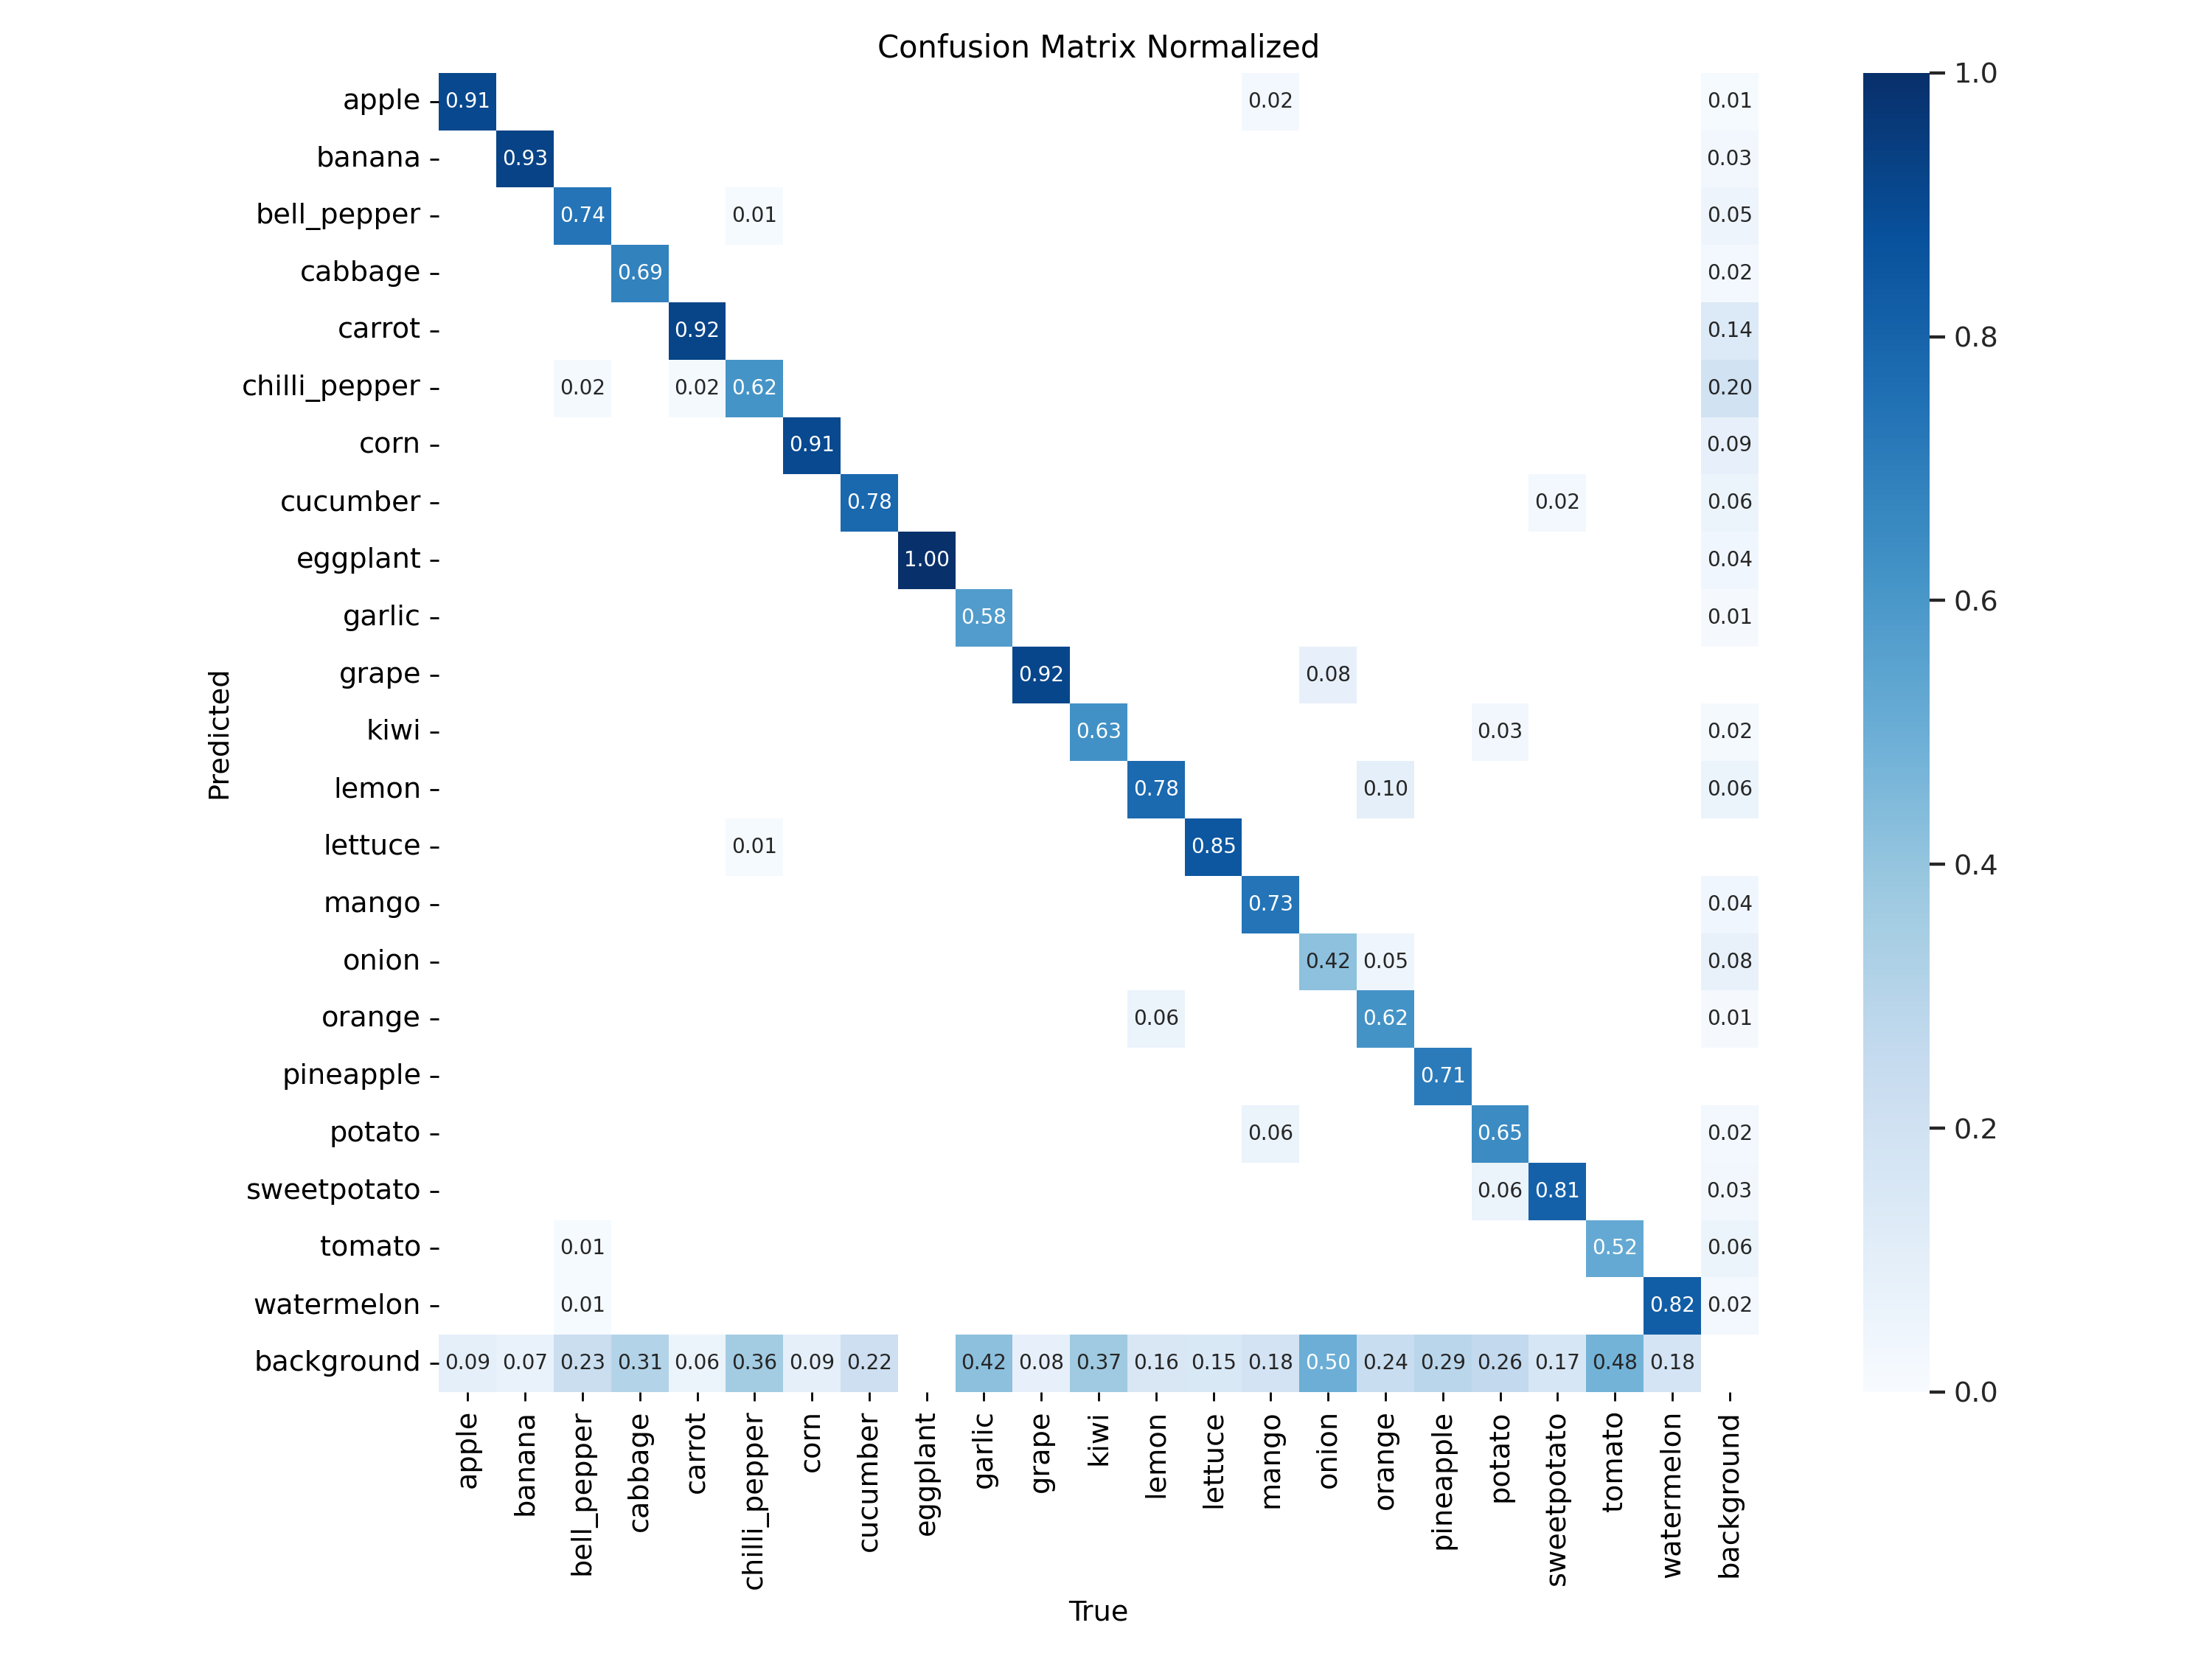
\includegraphics[width=0.8\linewidth]{../source/aws-img/yolov8/out/image/confusion_matrix_normalized.png}
    \caption{果实图像识别模型训练结果-混淆矩阵图}
    \label{fig:confusion_matrix_normalized}
\end{figure}

\section{服务接口设计}\label{sec:service}

本系统服务接口包含四个部分,分别是用户模块、果实模块、作业模块和称重模块。具体接口功能和路径设计如表\ref{tab:interface-user}、表\ref{tab:interface-produce}、表\ref{tab:interface-work}和表\ref{tab:interface-weigh}所示,接口风格均遵循 RESTful(Representational State Transfer, 即表现层状态转移)风格。

% 用户模块
\begin{table}[H]
\centering
\caption{用户模块接口设计}
\label{tab:interface-user}
\begin{tabular}{|c|c|c|}
\hline
接口名称 & 请求方法 & 接口路径 \\ \hline
用户获取个人信息 & GET & /user \\ \hline
管理员更新用户 & PUT & /user \\ \hline
管理员添加用户 & POST & /user \\ \hline
用户更新个人信息 & PUT & /user/me \\ \hline
用户登录 & POST & /user/login \\ \hline
管理员获取用户信息 & GET & /user/{uid} \\ \hline
管理员获取用户列表 & GET & /user/list \\ \hline
\end{tabular}
\end{table}

表\ref{tab:interface-user}显示了用户模块的接口设计,各接口以 /user 作为前缀。

% 果实模块
\begin{table}[H]
\centering
\caption{果实模块接口设计}
\label{tab:interface-produce}
\begin{tabular}{|c|c|c|}
\hline
接口名称 & 请求方法 & 接口路径 \\ \hline
根据名称获取果实 & GET & /produce \\ \hline
更新果实 & PUT & /produce \\ \hline
添加果实 & POST & /produce \\ \hline
获取果实 & GET & /produce/{id} \\ \hline
获取果实年产量 & GET & /produce/summary/year \\ \hline
获取果实分批产量 & GET & /produce/summary/work \\ \hline
获取果实列表 & GET & /produce/list \\ \hline
\end{tabular}
\end{table}

表\ref{tab:interface-produce}显示了果实模块的接口设计,各接口以 /produce 作为前缀。

% 作业模块
\begin{table}[H]
\centering
\caption{作业模块接口设计}
\label{tab:interface-work}
\begin{tabular}{|c|c|c|}
\hline
接口名称 & 请求方法 & 接口路径 \\ \hline
更新采摘作业 & PUT & /work \\ \hline
添加采摘作业 & POST & /work \\ \hline
获取采摘作业 & GET & /work/{id} \\ \hline
获取果实的采摘作业列表 & GET & /work/produce/{id}\\ \hline
获取采摘作业列表 & GET & /work/list \\ \hline
\end{tabular}
\end{table}

表\ref{tab:interface-work}显示了作业模块的接口设计,各接口以 /work 作为前缀。

% 称重模块
\begin{table}[H]
\centering
\caption{称重模块接口设计}
\label{tab:interface-weigh}
\begin{tabular}{|c|c|c|}
\hline
接口名称 & 请求方法 & 接口路径 \\\hline
更新电子秤信息 & PUT & /weigh/scale \\ \hline
添加电子秤 & POST & /weigh/scale \\\hline
添加称重记录 & POST & /weigh/record \\\hline
提交待处理称重记录 & POST & /weigh/record/todo \\\hline
获取待处理称重记录 & GET & /weigh/record/todo/list \\\hline
获取称重记录 & POST & /weigh/record/list \\\hline
添加称重结果监控者 & POST & /weigh/monitor \\\hline
获取员工各作业采摘量 & GET & /weigh/summary \\\hline
获取电子秤 & GET & /weigh/scale/{id} \\\hline
获取电子秤列表 & GET & /weigh/scale/list \\\hline
\end{tabular}
\end{table}

表\ref{tab:interface-weigh}显示了称重模块的接口设计,各接口以 /weigh 作为前缀。

\section{本章小结}
